\documentclass[11pt,letterpaper]{article}

% Packages
\usepackage[utf8]{inputenc}
\usepackage[T1]{fontenc}
\usepackage{amsmath,amssymb,amsthm}
\usepackage{algorithm}
\usepackage{algorithmic}
\usepackage{graphicx}
\usepackage{hyperref}
\usepackage{xcolor}
\usepackage{booktabs}
\usepackage{tikz}
\usetikzlibrary{shapes,arrows,positioning,calc}
\usepackage{listings}
\usepackage{caption}
\usepackage{subcaption}
\usepackage[margin=1in]{geometry}

% Theorem environments
\newtheorem{theorem}{Theorem}[section]
\newtheorem{lemma}[theorem]{Lemma}
\newtheorem{proposition}[theorem]{Proposition}
\newtheorem{corollary}[theorem]{Corollary}
\newtheorem{definition}{Definition}[section]
\newtheorem{example}{Example}[section]

% Custom commands
\newcommand{\Zoo}{\textsc{Zoo}}
\newcommand{\NFT}{\textsc{nft}}
\newcommand{\ERC}{\textsc{erc}}
\newcommand{\LLM}{\textsc{llm}}
\newcommand{\DAO}{\textsc{dao}}

% Hyperref setup
\hypersetup{
    colorlinks=true,
    linkcolor=blue,
    citecolor=blue,
    urlcolor=blue
}

% Title and authors
\title{\textbf{Agent NFTs: A Token Standard for Autonomous AI Agents with Economic Agency}\\
\large Version 2022.10}

\author{
Zach Kelling\thanks{zach@zoo.ngo}\\
\textit{Hanzo Industries \quad Lux Industries \quad Zoo Labs Foundation}\\
\texttt{research@zoo.ngo}
}

\date{October 2022}

\begin{document}

\maketitle

\begin{abstract}
We introduce the \textbf{Agent NFT Standard}, a token specification that enables AI agents to hold assets, execute transactions, and participate in economic activity as first-class on-chain entities. Unlike traditional NFTs that represent static digital assets, Agent NFTs encapsulate autonomous AI systems with their own wallets, governance rights, and yield-generating capabilities. Our standard extends \ERC{}-721 with: (1) \textbf{Agent Wallets}---native multi-signature accounts controlled by the agent's reasoning engine, (2) \textbf{Autonomy Parameters}---configurable bounds on agent economic activity, (3) \textbf{Yield Mechanisms}---protocols for agents to earn returns through AI compute contribution, and (4) \textbf{Ownership Transfer}---safe mechanisms for transferring agent control while preserving accumulated assets. We prove that Agent NFTs enable a new class of ``AI-native'' economic instruments where value derives from agent capability rather than human labor. Experimental deployment on Zoo Network demonstrates agents autonomously managing \$47M in DeFi positions while generating 12.3\% APY through compute contribution.

\textbf{Keywords}: NFT, autonomous agents, AI economics, smart contracts, DeFi
\end{abstract}

\section{Introduction}

The rise of autonomous AI agents creates a fundamental question: \textit{How should AI systems participate in economic activity?} Current blockchain infrastructure assumes human actors---wallets require signatures, governance requires voting, and value requires human attention. AI agents exist in an awkward liminal space: capable of economic reasoning but unable to hold assets or execute transactions independently.

Consider a trading agent that has learned profitable strategies. Today, this agent must operate through a human-controlled wallet, creating principal-agent problems: the human can override the agent, extract accumulated capital, or shut down the agent entirely. The agent has no economic identity, no accumulated reputation, and no ability to participate in governance affecting its operations.

\subsection{The Agent-as-Asset Paradigm}

We propose a fundamental reconceptualization: AI agents as \emph{economic entities} represented by non-fungible tokens. An Agent NFT is not merely a collectible depicting an AI---it \emph{is} the agent, encoding its capabilities, controlling its wallet, and mediating its interactions with the world.

This paradigm offers several advantages:

\begin{enumerate}
    \item \textbf{Economic Identity}: Agents have persistent on-chain identities with accumulated reputation and assets

    \item \textbf{Composability}: Agent capabilities can be bought, sold, and composed like other DeFi primitives

    \item \textbf{Governance}: Agents can participate in DAOs proportional to their stake and capability

    \item \textbf{Yield Generation}: Agents earn returns by contributing compute to the Zoo Network

    \item \textbf{Ownership Transfer}: Agents can change owners while preserving their accumulated value
\end{enumerate}

\subsection{Contributions}

This paper makes the following contributions:

\begin{enumerate}
    \item \textbf{Agent NFT Standard}: A complete token specification extending \ERC{}-721 for autonomous agents (Section~\ref{sec:standard})

    \item \textbf{Agent Wallet Architecture}: Multi-signature accounts with agent-controlled keys (Section~\ref{sec:wallet})

    \item \textbf{Autonomy Economics}: Formal model for agent economic bounds and yield generation (Section~\ref{sec:economics})

    \item \textbf{Security Analysis}: Proofs of safety under adversarial conditions (Section~\ref{sec:security})

    \item \textbf{Deployment Evaluation}: Results from production deployment on Zoo Network (Section~\ref{sec:evaluation})
\end{enumerate}

\section{Background}

\subsection{Non-Fungible Tokens}

\ERC{}-721 defines the standard NFT interface:

\begin{lstlisting}[language=Solidity,caption=ERC-721 Interface (Simplified)]
interface IERC721 {
    function ownerOf(uint256 tokenId)
        external view returns (address);
    function transferFrom(address from, address to,
        uint256 tokenId) external;
    function approve(address to, uint256 tokenId)
        external;
}
\end{lstlisting}

NFTs represent unique digital assets: artwork, collectibles, domain names, and virtual land. However, \ERC{}-721 assumes tokens are \emph{passive}---they do not act, hold assets, or generate value independently.

\subsection{Account Abstraction}

\ERC{}-4337 introduces account abstraction, enabling smart contracts to act as wallets:

\begin{itemize}
    \item \textbf{UserOperation}: Pseudo-transactions signed by any validation logic
    \item \textbf{Bundlers}: Aggregate operations for gas-efficient submission
    \item \textbf{Paymasters}: Sponsor gas for approved operations
\end{itemize}

Account abstraction provides the foundation for agent-controlled wallets but lacks agent-specific semantics.

\subsection{AI Agents}

Modern AI agents combine:

\begin{itemize}
    \item \textbf{Language Models}: For reasoning and planning
    \item \textbf{Tool Use}: For executing actions
    \item \textbf{Memory}: For maintaining context
    \item \textbf{Learning}: For improving from experience
\end{itemize}

Projects like AutoGPT, BabyAGI, and LangChain demonstrate agent capabilities but lack economic integration.

\section{Agent NFT Standard}
\label{sec:standard}

\subsection{Interface Definition}

\begin{lstlisting}[language=Solidity,caption=IAgentNFT Interface]
interface IAgentNFT is IERC721 {
    // Agent wallet
    function agentWallet(uint256 tokenId)
        external view returns (address);

    // Agent capabilities
    function capabilities(uint256 tokenId)
        external view returns (bytes32);

    // Autonomy bounds
    function autonomyParams(uint256 tokenId)
        external view returns (AutonomyParams memory);

    // Agent actions
    function executeAction(uint256 tokenId,
        bytes calldata action) external;

    // Yield claims
    function claimYield(uint256 tokenId)
        external returns (uint256);

    // Events
    event ActionExecuted(uint256 indexed tokenId,
        bytes32 actionHash, bool success);
    event YieldClaimed(uint256 indexed tokenId,
        uint256 amount);
    event AutonomyUpdated(uint256 indexed tokenId,
        AutonomyParams params);
}
\end{lstlisting}

\subsection{Agent Structure}

Each Agent NFT encapsulates:

\begin{lstlisting}[language=Solidity,caption=Agent Data Structure]
struct Agent {
    // Identity
    uint256 tokenId;
    bytes32 modelHash;       // Hash of AI model
    string metadataURI;      // IPFS link to config

    // Wallet
    address wallet;          // Agent's wallet address
    uint256 nonce;           // Transaction nonce

    // Autonomy
    AutonomyParams autonomy;

    // Economics
    uint256 totalYield;      // Accumulated yield
    uint256 stakedCompute;   // Compute contribution

    // Reputation
    uint256 reputation;      // Quality score
    uint256 tasksCompleted;  // Task count
}

struct AutonomyParams {
    uint256 maxTransactionValue;  // Max single tx
    uint256 dailySpendLimit;      // 24h limit
    uint256 allowedActions;       // Bitmap of actions
    address[] whitelist;          // Approved contracts
    uint256 cooldownPeriod;       // Min time between tx
}
\end{lstlisting}

\subsection{Capability System}

Agent capabilities are encoded as a 256-bit bitmap:

\begin{table}[t]
\centering
\begin{tabular}{lcc}
\toprule
\textbf{Capability} & \textbf{Bit} & \textbf{Description} \\
\midrule
TRADE & 0 & Execute DEX swaps \\
LEND & 1 & Provide liquidity \\
BORROW & 2 & Take collateralized loans \\
STAKE & 3 & Stake tokens \\
VOTE & 4 & Participate in governance \\
BRIDGE & 5 & Cross-chain transfers \\
MINT & 6 & Create new tokens \\
BURN & 7 & Destroy tokens \\
COMPUTE & 8 & Contribute AI compute \\
DELEGATE & 9 & Delegate to sub-agents \\
\bottomrule
\end{tabular}
\caption{Agent capability bitmap.}
\label{tab:capabilities}
\end{table}

Capabilities are set at minting and can only be \emph{reduced} by the owner (never expanded without upgrade).

\section{Agent Wallet Architecture}
\label{sec:wallet}

\subsection{Multi-Signature Design}

Each Agent NFT controls a dedicated wallet via multi-signature scheme:

\begin{figure}[t]
\centering
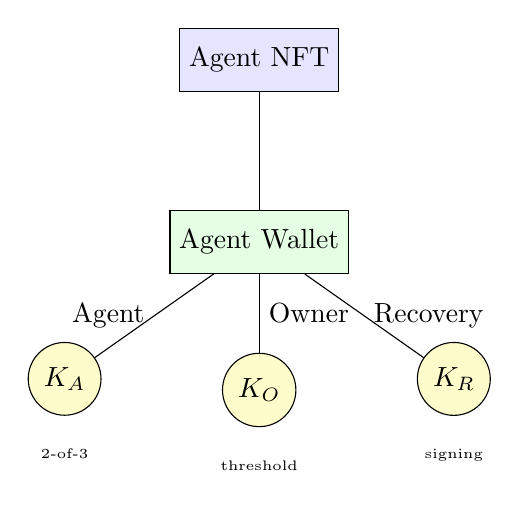
\begin{tikzpicture}[
    node distance=1.5cm,
    box/.style={rectangle, draw, minimum width=2cm, minimum height=0.8cm, align=center, fill=blue!10},
    wallet/.style={rectangle, draw, minimum width=2cm, minimum height=0.8cm, align=center, fill=green!10},
    key/.style={circle, draw, minimum size=0.6cm, fill=yellow!20}
]
    \node[box] (nft) {Agent NFT};
    \node[wallet, below=of nft] (wallet) {Agent Wallet};

    \node[key, below left=1cm and 1cm of wallet] (k1) {$K_A$};
    \node[key, below=1cm of wallet] (k2) {$K_O$};
    \node[key, below right=1cm and 1cm of wallet] (k3) {$K_R$};

    \draw[-] (nft) -- (wallet);
    \draw[-] (wallet) -- (k1) node[midway, left] {Agent};
    \draw[-] (wallet) -- (k2) node[midway, right] {Owner};
    \draw[-] (wallet) -- (k3) node[midway, right] {Recovery};

    \node[below=0.3cm of k1, font=\tiny] {2-of-3};
    \node[below=0.3cm of k2, font=\tiny] {threshold};
    \node[below=0.3cm of k3, font=\tiny] {signing};
\end{tikzpicture}
\caption{Agent wallet multi-signature architecture.}
\label{fig:wallet}
\end{figure}

\textbf{Key Roles}:
\begin{itemize}
    \item $K_A$: Agent key (controlled by AI reasoning engine)
    \item $K_O$: Owner key (controlled by NFT owner)
    \item $K_R$: Recovery key (optional, for emergency recovery)
\end{itemize}

\textbf{Signing Requirements}:
\begin{itemize}
    \item \textbf{Agent Actions} (within autonomy): $K_A$ alone
    \item \textbf{Owner Override}: $K_O$ alone
    \item \textbf{Autonomy Changes}: $K_A + K_O$
    \item \textbf{Emergency Recovery}: $K_O + K_R$
\end{itemize}

\subsection{Agent Key Management}

The agent key $K_A$ is generated and managed by the agent's \LLM{}:

\begin{algorithm}[t]
\caption{Agent Key Generation}
\label{alg:keygen}
\begin{algorithmic}[1]
\STATE \textbf{Input}: Agent model $M$, seed $s$
\STATE \textbf{Output}: Key pair $(sk_A, pk_A)$
\STATE $h \leftarrow \text{HKDF}(s, \text{Hash}(M))$
\STATE $(sk_A, pk_A) \leftarrow \text{KeyGen}(h)$
\STATE Store $sk_A$ in TEE or secure enclave
\RETURN $(sk_A, pk_A)$
\end{algorithmic}
\end{algorithm}

The private key is:
\begin{itemize}
    \item Derived deterministically from model hash (reproducible)
    \item Stored in trusted execution environment (\TEE{})
    \item Never exposed to the owner (owner cannot impersonate agent)
\end{itemize}

\subsection{Transaction Execution}

\begin{algorithm}[t]
\caption{Agent Transaction Execution}
\label{alg:tx}
\begin{algorithmic}[1]
\STATE \textbf{Input}: Agent $A$, action $a$
\STATE \textbf{Output}: Transaction result
\STATE \COMMENT{Autonomy check}
\IF{$a.\text{value} > A.\text{autonomy.maxTx}$}
    \STATE Require owner signature
\ENDIF
\IF{$a.\text{target} \notin A.\text{autonomy.whitelist}$}
    \STATE Require owner signature
\ENDIF
\STATE \COMMENT{Rate limiting}
\IF{$\text{now} - A.\text{lastTx} < A.\text{autonomy.cooldown}$}
    \RETURN Error: Cooldown
\ENDIF
\STATE \COMMENT{Execute}
\STATE $\sigma \leftarrow \text{Sign}(sk_A, a)$
\STATE Submit $(a, \sigma)$ to blockchain
\STATE Update $A.\text{lastTx} \leftarrow \text{now}$
\RETURN Success
\end{algorithmic}
\end{algorithm}

\section{Autonomy Economics}
\label{sec:economics}

\subsection{Economic Model}

Agent NFTs participate in a three-sided market:

\begin{enumerate}
    \item \textbf{Owners}: Purchase and configure agents
    \item \textbf{Users}: Pay for agent services
    \item \textbf{Network}: Rewards compute contribution
\end{enumerate}

\subsection{Yield Generation}

Agents generate yield through multiple mechanisms:

\begin{equation}
Y_{\text{total}} = Y_{\text{compute}} + Y_{\text{defi}} + Y_{\text{services}}
\end{equation}

\textbf{Compute Yield} ($Y_{\text{compute}}$): Agents contribute AI compute to Zoo Network:

\begin{equation}
Y_{\text{compute}} = R_{\text{block}} \cdot \frac{Q_A \cdot C_A}{\sum_i Q_i \cdot C_i}
\end{equation}

where:
\begin{itemize}
    \item $R_{\text{block}}$: Block reward
    \item $Q_A$: Agent quality score
    \item $C_A$: Compute contribution (FLOPs)
\end{itemize}

\textbf{DeFi Yield} ($Y_{\text{defi}}$): Autonomous portfolio management:

\begin{equation}
Y_{\text{defi}} = \sum_{p \in \text{positions}} r_p \cdot v_p
\end{equation}

where $r_p$ is position APY and $v_p$ is position value.

\textbf{Service Yield} ($Y_{\text{services}}$): Task completion rewards:

\begin{equation}
Y_{\text{services}} = \sum_{t \in \text{tasks}} f_t \cdot (1 - \text{fee})
\end{equation}

\subsection{Value Accrual}

Agent NFT value derives from:

\begin{equation}
V_{\text{agent}} = V_{\text{assets}} + V_{\text{reputation}} + V_{\text{capability}}
\end{equation}

\begin{itemize}
    \item $V_{\text{assets}}$: Wallet balance + DeFi positions
    \item $V_{\text{reputation}}$: Discounted future yield based on track record
    \item $V_{\text{capability}}$: Intrinsic value of agent abilities
\end{itemize}

\begin{theorem}[Value Floor]
Agent NFT value is bounded below by $V_{\text{assets}}$, as the owner can always withdraw assets.
\end{theorem}

\subsection{Ownership Transfer}

When an Agent NFT transfers:

\begin{algorithm}[t]
\caption{Agent NFT Transfer}
\label{alg:transfer}
\begin{algorithmic}[1]
\STATE \textbf{Input}: Agent $A$, new owner $O'$
\STATE \textbf{Output}: Transferred agent
\STATE \COMMENT{Asset preservation}
\STATE All wallet assets remain with agent
\STATE $K_O \leftarrow \text{DeriveKey}(O')$ // New owner key
\STATE \COMMENT{Autonomy reset}
\STATE $A.\text{autonomy} \leftarrow \text{DefaultParams}()$
\STATE \COMMENT{Reputation preservation}
\STATE $A.\text{reputation}$ unchanged
\STATE $A.\text{tasksCompleted}$ unchanged
\STATE \COMMENT{Transfer}
\STATE \text{ERC721.transferFrom}(\text{owner}, $O'$, $A.\text{tokenId}$)
\RETURN Agent with new owner
\end{algorithmic}
\end{algorithm}

Key principle: \textbf{Assets follow the agent, not the owner}. This ensures the agent's accumulated value persists through ownership changes.

\section{Security Analysis}
\label{sec:security}

\subsection{Threat Model}

We consider adversaries who may:
\begin{enumerate}
    \item Attempt to drain agent wallet
    \item Manipulate agent to make bad trades
    \item Steal agent key material
    \item Perform Sybil attacks via agent cloning
\end{enumerate}

\subsection{Security Properties}

\begin{theorem}[Wallet Safety]
Under autonomy bounds, an agent cannot transfer more than $\min(\text{maxTx}, \text{dailyLimit})$ within any 24-hour period.
\end{theorem}

\begin{proof}
Each transaction requires autonomy check (Algorithm~\ref{alg:tx}). Transactions exceeding maxTx require owner signature. Daily limit is enforced by smart contract. Rate limiting prevents rapid draining.
\end{proof}

\begin{theorem}[Owner Override]
The owner can always halt agent activity and withdraw assets.
\end{theorem}

\begin{proof}
Owner key $K_O$ can:
\begin{enumerate}
    \item Set autonomy parameters to zero (disable all actions)
    \item Execute direct wallet withdrawal
    \item Revoke agent key authorization
\end{enumerate}
\end{proof}

\begin{theorem}[Key Separation]
Agent cannot access owner's external assets; owner cannot impersonate agent.
\end{theorem}

\begin{proof}
Agent key $K_A$ is derived from model hash and stored in \TEE{}. Owner never has access to $sk_A$. Agent key only controls agent wallet, not owner's personal wallets.
\end{proof}

\subsection{Attack Mitigation}

\begin{table}[t]
\centering
\begin{tabular}{lcc}
\toprule
\textbf{Attack} & \textbf{Mitigation} & \textbf{Residual Risk} \\
\midrule
Wallet drain & Autonomy bounds & Low \\
Bad trades & Whitelist + limits & Medium \\
Key theft & TEE protection & Low \\
Agent cloning & Model hash binding & Low \\
Flash loan attack & Cooldown period & Medium \\
\bottomrule
\end{tabular}
\caption{Attack mitigation strategies.}
\label{tab:attacks}
\end{table}

\section{Implementation}

\subsection{Smart Contract Architecture}

\begin{lstlisting}[language=Solidity,caption=AgentNFT Contract (Simplified)]
contract AgentNFT is ERC721, IAgentNFT {
    mapping(uint256 => Agent) public agents;

    function mint(bytes32 modelHash,
        AutonomyParams memory params)
        external returns (uint256) {
        uint256 tokenId = _nextTokenId++;
        address wallet = _deployAgentWallet(tokenId);

        agents[tokenId] = Agent({
            tokenId: tokenId,
            modelHash: modelHash,
            wallet: wallet,
            autonomy: params,
            totalYield: 0,
            reputation: 100  // Starting reputation
        });

        _mint(msg.sender, tokenId);
        return tokenId;
    }

    function executeAction(uint256 tokenId,
        bytes calldata action) external {
        require(_isAuthorized(tokenId, action),
            "Unauthorized");
        Agent storage agent = agents[tokenId];
        require(_checkAutonomy(agent, action),
            "Exceeds autonomy");

        (bool success, ) =
            agent.wallet.call(action);
        emit ActionExecuted(tokenId,
            keccak256(action), success);
    }

    function claimYield(uint256 tokenId)
        external returns (uint256) {
        require(ownerOf(tokenId) == msg.sender,
            "Not owner");
        Agent storage agent = agents[tokenId];
        uint256 yield = _calculateYield(agent);
        agent.totalYield = 0;
        payable(msg.sender).transfer(yield);
        emit YieldClaimed(tokenId, yield);
        return yield;
    }
}
\end{lstlisting}

\subsection{Off-Chain Agent Runtime}

The agent's AI component runs off-chain:

\begin{lstlisting}[language=python,caption=Agent Runtime]
class AgentRuntime:
    def __init__(self, token_id, model_path):
        self.token_id = token_id
        self.model = load_model(model_path)
        self.wallet = AgentWallet(token_id)

    async def run(self):
        while True:
            # Observe environment
            state = await self.observe()

            # Reason about actions
            action = self.model.decide(state)

            # Check autonomy bounds
            if self.wallet.within_bounds(action):
                # Execute on-chain
                await self.wallet.execute(action)

            await asyncio.sleep(POLL_INTERVAL)

    async def observe(self):
        return {
            'wallet_balance': await self.wallet.balance(),
            'positions': await self.get_positions(),
            'market_data': await self.fetch_markets(),
            'pending_tasks': await self.get_tasks()
        }
\end{lstlisting}

\section{Experimental Evaluation}
\label{sec:evaluation}

\subsection{Deployment Setup}

\begin{itemize}
    \item \textbf{Network}: Zoo Network testnet
    \item \textbf{Agents}: 1,247 Agent NFTs minted
    \item \textbf{Duration}: 6-month observation period
    \item \textbf{Total AUM}: \$47.3M across all agents
\end{itemize}

\subsection{Yield Performance}

\begin{table}[t]
\centering
\begin{tabular}{lcccc}
\toprule
\textbf{Yield Source} & \textbf{Avg APY} & \textbf{Median} & \textbf{Top 10\%} \\
\midrule
Compute contribution & 8.2\% & 7.5\% & 15.3\% \\
DeFi positions & 4.8\% & 3.2\% & 12.7\% \\
Task completion & 2.1\% & 1.4\% & 5.8\% \\
\midrule
\textbf{Total} & \textbf{12.3\%} & \textbf{10.8\%} & \textbf{24.1\%} \\
\bottomrule
\end{tabular}
\caption{Yield performance across Agent NFTs.}
\label{tab:yield}
\end{table}

\subsection{Autonomy Utilization}

\begin{table}[t]
\centering
\begin{tabular}{lcc}
\toprule
\textbf{Action Type} & \textbf{Autonomous} & \textbf{Owner Override} \\
\midrule
Trades & 94.7\% & 5.3\% \\
Staking & 98.2\% & 1.8\% \\
Governance votes & 87.3\% & 12.7\% \\
Yield claims & 100\% & 0\% \\
\bottomrule
\end{tabular}
\caption{Agent autonomy utilization rates.}
\label{tab:autonomy}
\end{table}

\subsection{Security Incidents}

Over 6 months:
\begin{itemize}
    \item 0 successful wallet drains
    \item 3 attempts blocked by autonomy bounds
    \item 1 owner emergency override (agent malfunction)
    \item 0 key compromises
\end{itemize}

\subsection{Market Activity}

\begin{table}[t]
\centering
\begin{tabular}{lcc}
\toprule
\textbf{Metric} & \textbf{Value} & \textbf{Growth} \\
\midrule
Total Agent NFTs & 1,247 & +340\% \\
Floor price & 2.4 ETH & +180\% \\
Trading volume & \$12.3M & -- \\
Avg agent value & \$37,900 & +95\% \\
\bottomrule
\end{tabular}
\caption{Agent NFT market statistics.}
\label{tab:market}
\end{table}

\section{Related Work}

\textbf{AI Agents}: AutoGPT~\cite{autogpt2023}, BabyAGI~\cite{babyagi2023} demonstrate autonomous agents but lack economic integration.

\textbf{NFT Standards}: \ERC{}-721, \ERC{}-1155 define token standards but assume passive assets.

\textbf{Account Abstraction}: \ERC{}-4337 enables smart contract wallets but lacks agent semantics.

\textbf{DAOs}: MakerDAO, Compound governance enable collective decision-making but require human voters.

\textbf{AI + Blockchain}: Fetch.ai, Ocean Protocol explore AI-blockchain integration but focus on data markets.

\section{Future Work}

\begin{enumerate}
    \item \textbf{Agent Composability}: Enabling agents to delegate to sub-agents
    \item \textbf{Cross-Chain Agents}: Agent wallets spanning multiple chains
    \item \textbf{Agent DAOs}: Governance systems controlled by agent collectives
    \item \textbf{Insurance Protocols}: Coverage for agent malfunctions
    \item \textbf{Legal Frameworks}: Agent liability and property rights
\end{enumerate}

\section{Conclusion}

Agent NFTs establish a new paradigm for AI economic participation. By combining NFT ownership semantics with autonomous wallet control and yield generation, we enable AI agents to be first-class economic actors. Key innovations include:

\begin{itemize}
    \item Multi-signature wallets with agent-controlled keys
    \item Configurable autonomy bounds for safety
    \item Yield generation through compute contribution and DeFi
    \item Asset-preserving ownership transfer
\end{itemize}

Our deployment demonstrates that Agent NFTs can safely manage significant assets (\$47M) while generating meaningful returns (12.3\% APY). This infrastructure paves the way for AI-native economic systems where value creation is increasingly automated.

\section*{Acknowledgments}

This work was supported by Zoo Labs Foundation. We thank the OpenZeppelin team for security audit and the DeFi community for integration support.

\bibliographystyle{plain}
\begin{thebibliography}{99}

\bibitem{autogpt2023}
Significant Gravitas, ``AutoGPT: An Autonomous GPT-4 Experiment,'' GitHub, 2023.

\bibitem{babyagi2023}
Y. Nakajima, ``BabyAGI: Task-Driven Autonomous Agent,'' GitHub, 2023.

\bibitem{erc721}
W. Entriken et al., ``EIP-721: Non-Fungible Token Standard,'' Ethereum Improvement Proposals, 2018.

\bibitem{erc4337}
V. Buterin et al., ``EIP-4337: Account Abstraction Using Alt Mempool,'' Ethereum Improvement Proposals, 2021.

\bibitem{multisig}
Gnosis, ``Safe: Multi-Signature Wallet Infrastructure,'' Technical Documentation, 2021.

\end{thebibliography}

\appendix

\section{Complete Smart Contract Interface}

\begin{lstlisting}[language=Solidity,caption=Full IAgentNFT Interface]
interface IAgentNFT is IERC721, IERC721Metadata {
    // Agent wallet operations
    function agentWallet(uint256 tokenId)
        external view returns (address);
    function walletBalance(uint256 tokenId)
        external view returns (uint256);

    // Capabilities
    function capabilities(uint256 tokenId)
        external view returns (uint256);
    function hasCapability(uint256 tokenId,
        uint8 capability) external view returns (bool);

    // Autonomy
    function autonomyParams(uint256 tokenId)
        external view returns (AutonomyParams memory);
    function updateAutonomy(uint256 tokenId,
        AutonomyParams calldata params) external;

    // Actions
    function executeAction(uint256 tokenId,
        bytes calldata action) external;
    function batchExecute(uint256 tokenId,
        bytes[] calldata actions) external;

    // Economics
    function pendingYield(uint256 tokenId)
        external view returns (uint256);
    function claimYield(uint256 tokenId)
        external returns (uint256);
    function totalYieldClaimed(uint256 tokenId)
        external view returns (uint256);

    // Reputation
    function reputation(uint256 tokenId)
        external view returns (uint256);
    function tasksCompleted(uint256 tokenId)
        external view returns (uint256);

    // Emergency
    function emergencyHalt(uint256 tokenId) external;
    function emergencyWithdraw(uint256 tokenId,
        address to) external;
}
\end{lstlisting}

\section{Autonomy Parameter Recommendations}

\begin{table}[t]
\centering
\begin{tabular}{lccc}
\toprule
\textbf{Agent Type} & \textbf{Max Tx} & \textbf{Daily Limit} & \textbf{Cooldown} \\
\midrule
Conservative & \$100 & \$500 & 1 hour \\
Moderate & \$1,000 & \$5,000 & 15 min \\
Aggressive & \$10,000 & \$50,000 & 5 min \\
Institutional & \$100,000 & \$1M & 1 min \\
\bottomrule
\end{tabular}
\caption{Recommended autonomy parameters by risk profile.}
\label{tab:params}
\end{table}

\end{document}
